\documentclass[a4paper,titlepage]{article}

%PACKAGES
\usepackage[utf8]{inputenc}
\usepackage[T1]{fontenc}
\usepackage[english]{babel}
\usepackage{amsmath}
\usepackage{amssymb}
\usepackage{mathrsfs}
\usepackage{fancyhdr}
\usepackage{lmodern}
\usepackage{graphicx}
\usepackage{geometry}
\usepackage{fancybox}
\usepackage{textcomp}

%Symbole euro
\usepackage{eurosym}

%Listings : affichage code
\usepackage{listings}


%Elements de la page de garde
\begin{document}

\begin{titlepage}

\begin{figure}
\centering

\includegraphics[width=5cm]{logo-ulg.png}
\end{figure}



\title{
\vspace{0.2cm}
\LARGE{\textbf{Project 2 - Developing a web-based SNMP browser }} \\ \textsc{Managing and securing computer networks}
\author{\textbf{Floriane Magera} \small{(S111295})\\\textbf{Fabrice Servais} \small{(S111093})}\\
\date{April 15, 2015}
\rule{15cm}{1.5pt}
}

%\geometry{hmargin=2.5cm}
\end{titlepage}

%DOCUMENT
\pagestyle{fancy}
\lhead{Project 2 - MIB browser}
\rhead{Managing and securing computer networks}

%Page de garde
\maketitle

\section{Detecting the agents}
To enhance the previous script, we took the one provided to us and modify it in order to allow it to write the results in the XML, as in the first part of the project.

\paragraph{}

The files had been put in the \texttt{public\_html/discover}. To run the CRON job, one can use the command:
\begin{center}
	\texttt{crontab cron.txt}
\end{center}
or uniquely the script for testing purpose: 
\begin{center}
	\texttt{python3 discover.py}
\end{center}
The result will be put in \texttt{public\_html/agents.xml}.


\section{Application}
Our website is available at the page : 
\begin{center}
	http://bee.run.montefiore.ulg.ac.be/\textasciitilde nms01/
\end{center}
To develop our application, we used the MVC pattern.

\subsection{Model}

The model is implemented by a SQLite database and retains the agents and the list of objects for each agent, which allows a quite fast retrieval of information, it is a cache. This database has a timeout of two hours, if we try to access it after that, it will retrieve the information again and update the cache:
\begin{itemize}
	\item For the agents, the list is stored in the \texttt{/model} directory in a XML file, which is read before inserting the agents in the database. The XML file is indeed adding one more step, from retrieving the agents to store them in the database. An improvement could be to store them directly in the database, however, in the first part of the project, we stored them in the XML format. To keep coherence (and by lack of time), we kept this transitional and read from it to populate the database.

	\item To list of OID's contained in an agent are got by running a serie of \texttt{snmpgetnext}, beginning at the root. We did not used \texttt{snmpwalk} because it seems that it retrieved less objects than \texttt{snmpgetnext}. These objects are directly stored in the cache as the retrieval is finished. Same as the agents' cache, it is refreshed after two hours. In the database, an agent is always recognized by the 4-tuple (ip, port, version, sec\_name). We also provide phpLiteAdmin to see in a more easier way the content of the database\footnote{http://bee.run.montefiore.ulg.ac.be/\textasciitilde nms01/phpliteadmin.php - Password: admin}.
	\paragraph{}
	When the list is returned to the controller, the array containing the OID's is exploded to form a tree-structured array, an "OID-tree like". For exemple, \texttt{array("1.2.1" => "a", "1.2.2" => "b")} becomes (more or less) \texttt{array("1" => array("2" => array("1" => "a", "2" => "b")))}. This function \texttt{explodeTree(\$array, \$delimiter = '.', \$baseval = false)} comes from an external source\footnote{http://kvz.io/blog/2007/10/03/convert-anything-to-tree-structures-in-php/}, making the development faster since we do not have to solve the problem ourselves.
\end{itemize}

The scheme of the database is shown \textsc{Figure} \ref{db}. Note that the foreign key constraints are not implemented.
\begin{figure}
	\centering
	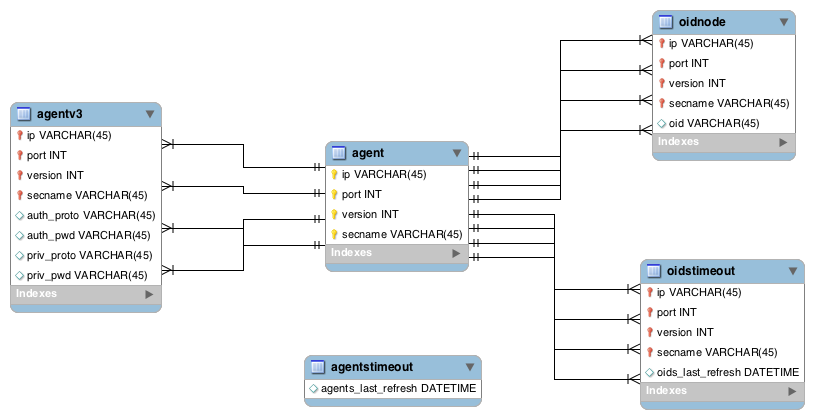
\includegraphics[scale=0.55]{db.png}
	\caption{Database structure}
	\label{db}
\end{figure}

\subsection{Controller}
The controller processes the client requests by retrieving from the model the information needed. In the case of the request of an OID value, it sends the SNMP request directly in the network.

\paragraph{}

We tried to make the requests to the database as light as possible, that is why we only retrieve all the mib list for an agent, even if we know the OID of the requested object. The model transforms the list in a form of tree, which allows efficient access from the controller.

\paragraph{}

We also decided that the information needed to identify an SNMP agent are its ip address, its port number, the SNMP version used and the community name. The other informations about SNMPv3 agents are kept local and never communicated to the client, it is a (maybe too) simple way to avoid communicating the passwords to the client. 


\subsection{View}
The view is simple, it displays the data the controller collected. 



\section{Feedback} 
We think the projects were interesting, it allowed us to learn new things : we had never coded in python, neither heard about cron jobs, and creating a website is always a good exercice, as we don't do it often, but we think it is essential to have some experience in that field too.

\paragraph{}

The SNMP subject is sure important and helped us realise that it is not "simple" as its name could let us think and it is good to have the opportunity to have some "hands-on" experience of SNMP. However, we would also have enjoyed a subject more related to security, even if we have the projects of the course "Introduction to computer securiy".
\end{document}
